\chapter{Review of Image-Based Approaches in Wheat Disease Identification}

\section{Introduction}
In recent years, image-based approaches leveraging advances in deep learning have emerged as powerful tools for the early detection and classification of wheat diseases. These methods rely on the visual symptoms present on wheat leaves, stems, or spikes, captured through images and analyzed using automated algorithms.

This chapter provides a comprehensive review of existing image-based approaches for wheat disease identification. It begins with an exploration of data collection and preprocessing techniques, including data augmentation strategies to enhance model robustness. The chapter then delves into different classification models and frameworks used for disease recognition. Finally, it highlights the current limitations and identifies research gaps that still need to be addressed to improve the accuracy, scalability, and real-world applicability of these systems.

\section{Approaches in Data Collection and Preprocessing }
This section discusses various methods employed in the literature for gathering data, handling challenges such as low-quality or irrelevant images, and preprocessing techniques that prepare datasets for effective utilization in classification and detection tasks.

\subsection{Data Collection}
The initial and foundational step in developing deep learning models for wheat disease classification is the acquisition of high-quality and diverse image data. This data can be sourced through various means, including manual and automated methods. Common sources include drone-mounted or mobile device cameras, which allow for the real-time capture of wheat leaf images under natural field conditions. Public datasets also play a crucial role; for instance, the "Wheat Leaf Dataset" available on Kaggle, utilized by \parencite{ramadan2024improving}, and the "Wheat Disease Detection" dataset, employed by \parencite{reis2024integrated}, offer extensive repositories of labeled images. In addition to these, hybrid data collection strategies are often employed. \parencite{hassan2024wheat}, for example, combined images obtained from field visits, Kaggle datasets, and internet sources to enrich their training data. This diversity in data sources helps improve the robustness and generalization capability of the resulting models.


\subsection{Data Preprocessing}
Data preprocessing plays a crucial role in improving the quality and relevance of input images for deep learning models. This process typically begins with the elimination of low-quality images where disease symptoms are poorly visible \parencite{yao2024yolo} and the cropping of extraneous image regions to concentrate on areas of diagnostic interest. To further enhance the visual quality, advanced contrast enhancement techniques such as Contrast Limited Adaptive Histogram Equalization (CLAHE), contrast stretching, and the hypercolumn technique (Figure~\ref{fig:CLAHE}) are commonly employed to improve image contrast and brightness, as discussed by \parencite{reis2024integrated} and \parencite{fang2023lightweight}. These methods significantly improve image contrast and brightness, making subtle disease features more discernible and thereby facilitating more accurate classification. Additionally, to isolate the region of interest and reduce background noise, methods such as background removal, color thresholding, and edge detection are utilized \parencite{alharbi2023wheat}, ensuring that only the most relevant image features are presented to the model.


\begin{figure}[H] % 'H' needs \usepackage{float}
    \centering
    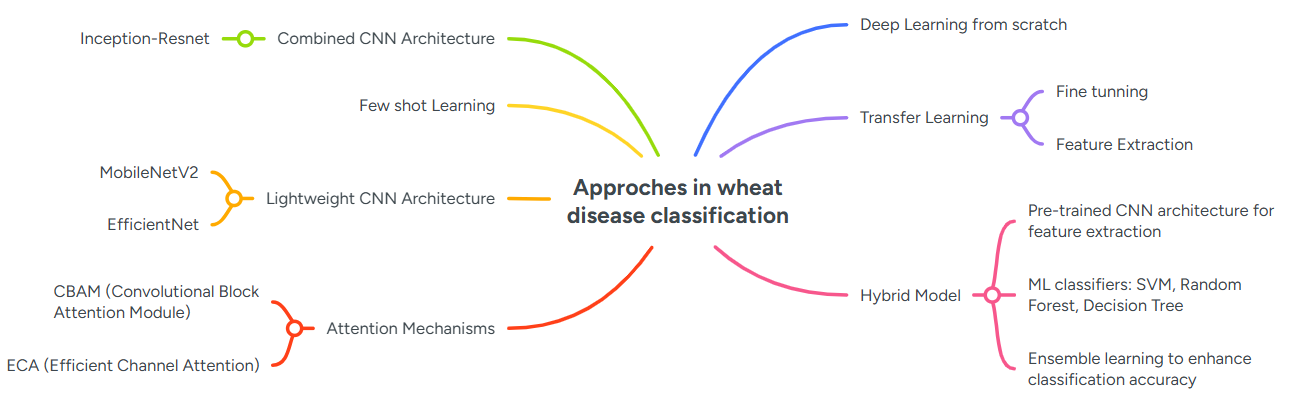
\includegraphics[width=0.8\textwidth]{chapters/chapter3/images/Figure01.png}
    \caption{Sub-data samples of the wheat disease original dataset obtained by the CLAHE, Contrast stretching, and hypercolumn technique \parencite{reis2024integrated}.}
    \label{fig:CLAHE}
\end{figure}

\subsection{Data augmentation}

Data augmentation is extensively employed to mitigate class imbalance and enhance dataset diversity, thereby improving the generalization capabilities of deep learning models. Common augmentation techniques include random rotations, cropping, zooming, flipping, and contrast adjustments (Figure~\ref{fig:Dataaugmentation}), which artificially expand the training dataset by introducing varied visual representations of the original images \parencite{nagpal2024hybrid,hassan2024wheat,nigam2023deep}.

\begin{figure}[H] % 'H' needs \usepackage{float}
    \centering
    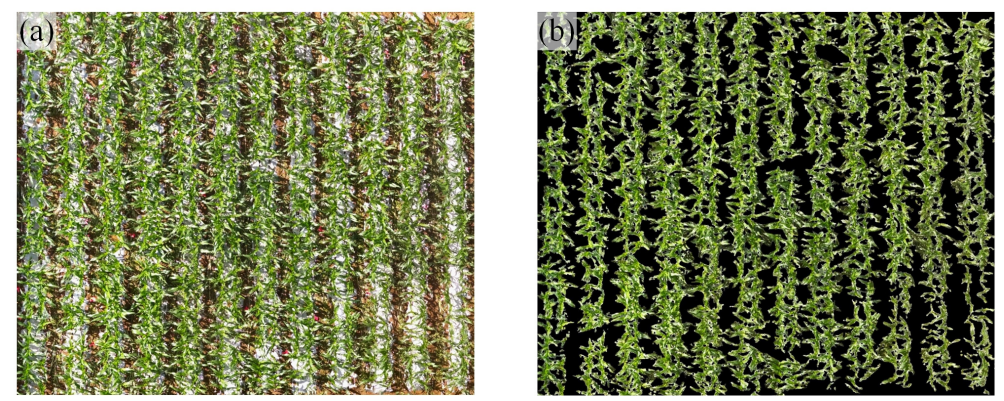
\includegraphics[width=0.6\textwidth]{chapters/chapter3/images/Figure02.png}
    \caption{Data augmentation techniques \parencite{nagpal2024hybrid}.}
    \label{fig:Dataaugmentation}
\end{figure}

\parencite{ramadan2024improving} use four augmentation techniques enhance dataset diversity and address class imbalance: CycleGAN, which generates realistic synthetic images through unpaired image-to-image translation; ADASYN, which adaptively oversamples difficult minority class instances; SMOTE, which creates synthetic samples by interpolating between minority class neighbors; and SMOTE-Tomek, a hybrid method that combines SMOTE with Tomek links to both oversample and remove noisy boundary samples.




\section{Approaches in Wheat Disease Classification}

Various classification models have been employed in the literature to address wheat disease classification effectively. These approaches, preprocessing techniques, datasets, classification categories, and results are summarized in Table~\ref{tab:Table 01}, which provides a comparative overview of the most recent and relevant studies in this domain.

\textbf{Transfer Learning Approaches:} \parencite{jiang2022evaluation} compares three CNN training strategies for wheat disease identification (Figure~\ref{fig:TrainingStrategies}): training from scratch, fixed feature extraction, and transfer learning with fine-tuning.

\begin{itemize}
  \item \textbf{Training from scratch:} The entire CNN is trained from the beginning with randomly initialized weights using only the target dataset (FWDI). This approach allows full customization but requires a large amount of data and significant computational power.

  \item \textbf{Fixed feature extraction:} In this strategy, a pre-trained CNN is employed as a fixed feature extractor, where all convolutional layers are frozen to preserve the learned representations, and only the final classification layers—such as the fully connected, batch normalization, and softmax layers are retrained on the target dataset. A similar approach was employed by \parencite{nigam2023deep}, who fine-tuned a pre-trained EfficientNet model on their custom WheatRust21 dataset for wheat rust classification, achieving an impressive accuracy of 99.35\%.

  \item \textbf{Transfer learning with fine-tuning:} This approach involves partially or fully retraining a pre-trained CNN on the target dataset, enabling the model to adapt learned features to the specific characteristics of the new domain. By leveraging representations learned from a large, diverse source dataset, fine-tuning enhances the model’s ability to capture domain-specific patterns in the target dataset. \parencite{jiang2022evaluation} applied this strategy, achieving 92.5\% accuracy on the FWDI and PlantVillage datasets using InceptionV3. Similarly, \parencite{ramadan2024improving} fine-tuned pre-trained CNNs such as DenseNet121, ResNet50V2, MobileNetV2, and Xception for wheat leaf disease classification, using both augmented and non-augmented datasets, and achieved 100\% accuracy in predicting three classes (healthy, stripe rust, or septoria), further validating the effectiveness of fine-tuning in this domain.
\end{itemize}


\begin{figure}[H] 
    \centering
    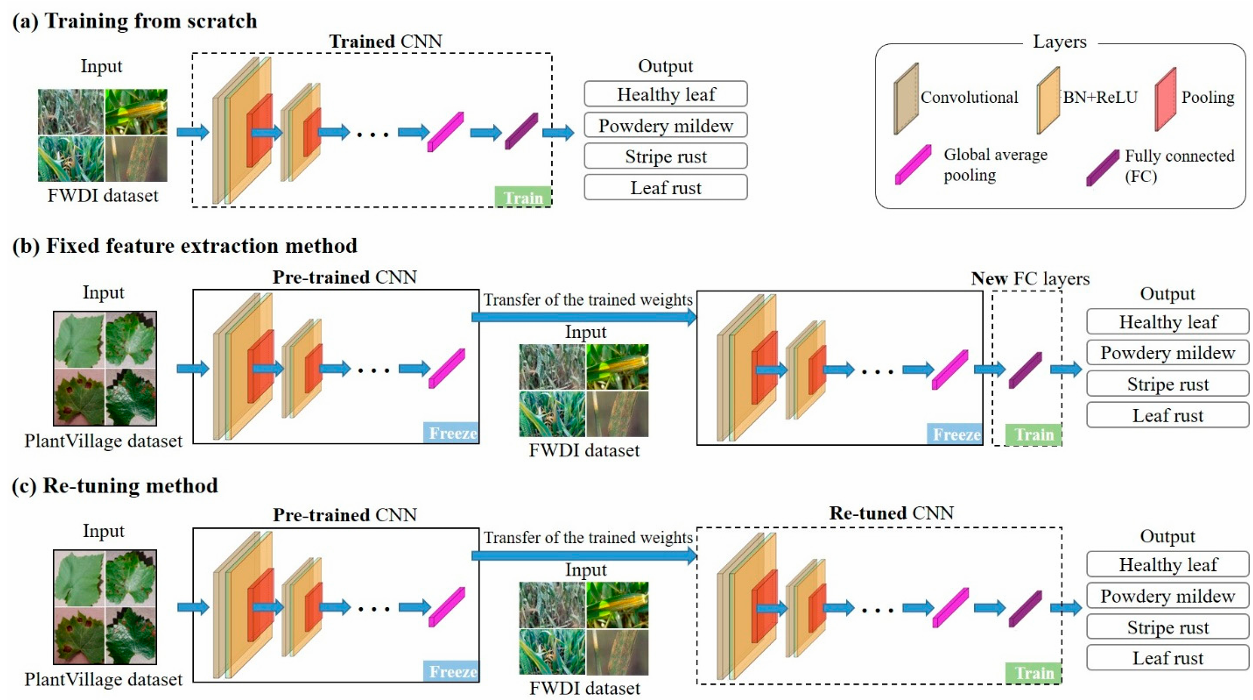
\includegraphics[width=1\textwidth]{chapters/chapter3/images/Figure03.png}
    \caption{Training strategies of a convolutional neural network (CNN) \parencite{jiang2022evaluation}.}
    \label{fig:TrainingStrategies}
\end{figure}



\textbf{Hybrid Models:} \parencite{nagpal2024hybrid} Introduced a hybrid model (Figure~\ref{fig:hybridframework}) that combines deep learning and traditional machine learning for image classification. Features are extracted from images using two pre-trained CNN models, MobileNet and DenseNet, and then concatenated. Particle Swarm Optimization (PSO) is applied for dimensionality reduction. Finally, the reduced features are fed into traditional classifiers (RF, SVM, DT) for training and prediction, achieving an accuracy of 98.89\% across four classes.


\begin{figure}[H] 
    \centering
    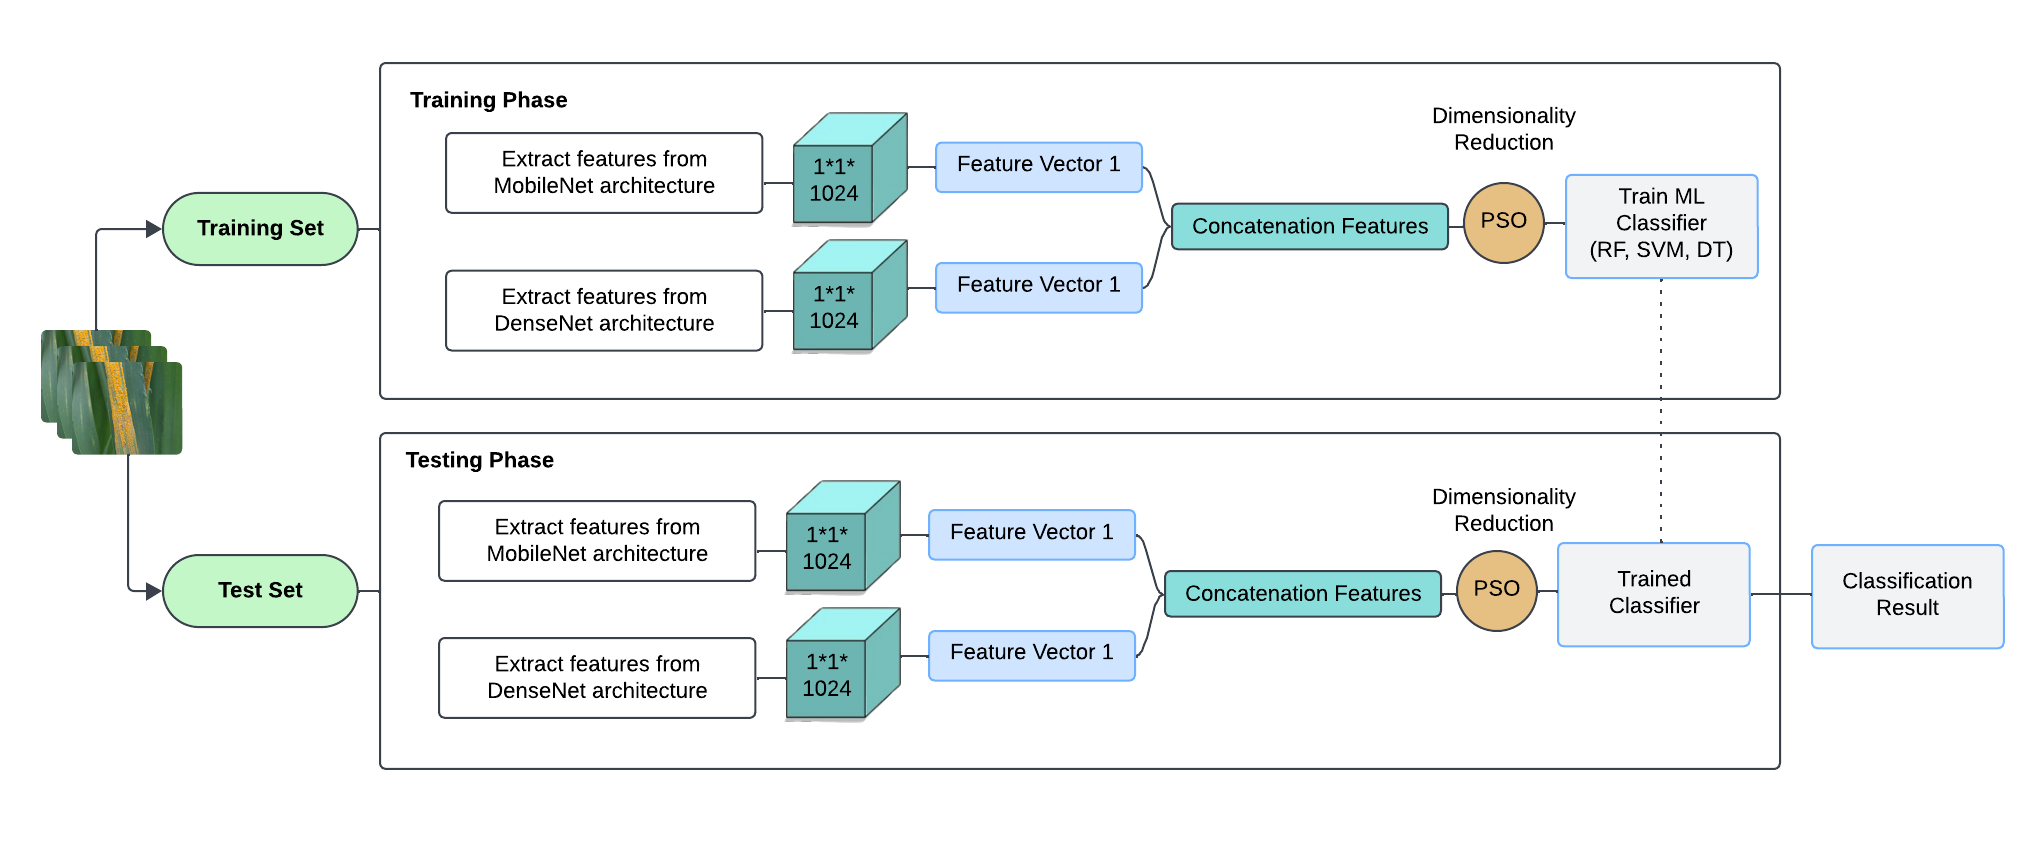
\includegraphics[width=1\textwidth]{chapters/chapter3/images/Figure04.png}
    \caption{The architecture of the hybrid framework \parencite{nagpal2024hybrid}.}
    \label{fig:hybridframework}
\end{figure}









\textbf{Custom Deep Convolutional Networks:} \parencite{goyal2021leaf} proposed a custom deep convolutional neural network (Figure~\ref{fig:CustomDeepCN}) specifically designed for wheat disease classification. The architecture comprises 21 convolutional layers, 7 max-pooling layers, and 3 fully connected layers. Activation functions used include ReLU and Leaky ReLU in the convolutional layers, while the fully connected layers employ ReLU, followed by a SoftMax classifier for multi-class output. The model was trained on a dataset of over 12,000 labeled RGB images covering 10 distinct wheat disease classes and achieved an accuracy of 97.88\%. 

\begin{figure}[H] 
    \centering
    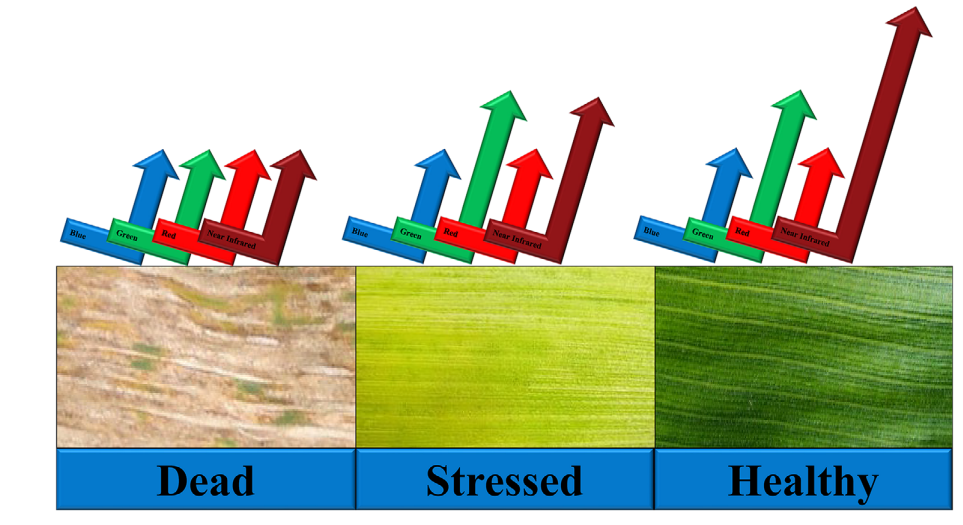
\includegraphics[width=0.8\textwidth]{chapters/chapter3/images/Figure05.png}
    \caption{The proposed deep convolutional neural network \parencite{goyal2021leaf}.}
    \label{fig:CustomDeepCN}
\end{figure}



\textbf{Few-Shot Learning:} \parencite{alharbi2023wheat} implemented a few-shot learning approach (Figure~\ref{fig:Few-shot}) using a Siamese network with EfficientNetB0 as a shared feature extractor to process both support and query images, generating feature embeddings for each. The support set contains a small number of labeled examples per class, while the query set includes unlabeled images to be classified. The Siamese structure ensures that the same feature extraction process is applied to both sets, enabling meaningful comparison. This model achieved an accuracy of 93.19\% in classifying 18 types of wheat diseases.


\begin{figure}[H] 
    \centering
    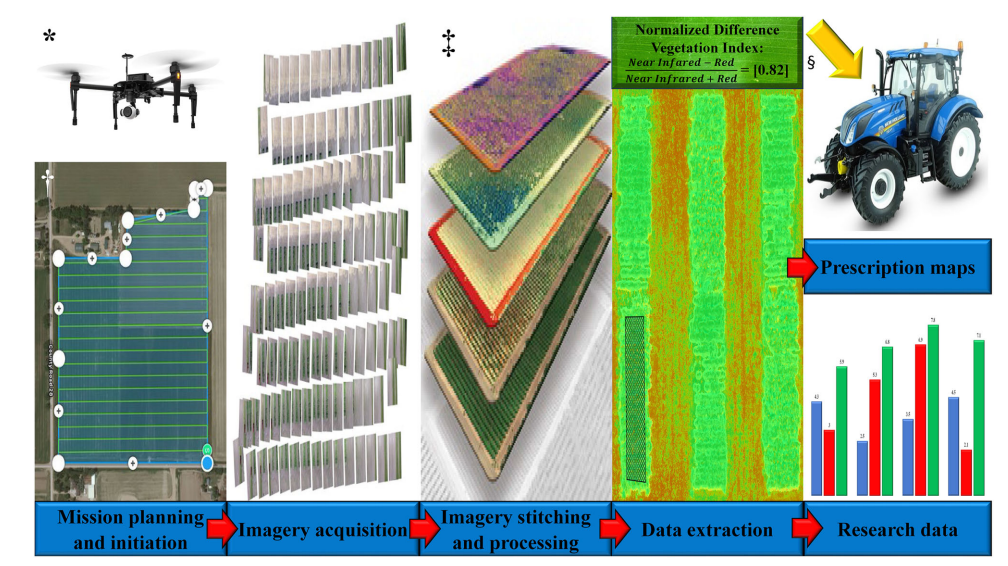
\includegraphics[width=0.9\textwidth]{chapters/chapter3/images/Figure06.png}
    \caption{Architecture diagram of a Few-shot Learning-based network \parencite{alharbi2023wheat}.}
    \label{fig:Few-shot}
\end{figure}


\textbf{Lightweight CNNs for Efficient Classification:} \parencite{fang2023lightweight} introduced a lightweight multiscale CNN model optimized for mobile and edge computing applications. By integrating Inception modules with residual blocks and attention mechanisms like Convolutional Block Attention Model (CBAM) and Efficient Channel Attention (ECA), the model enhanced feature extraction while reducing computational costs, achieving 98.78\% accuracy on wheat disease classification tasks​. Likewise, \parencite{jouini2023wheat} proposed a deep learning approach using MobileNetV2 and EfficientNet variants to build a lightweight yet accurate CNN-based model for wheat leaf disease detection in smart agriculture, achieving 94\% test accuracy.




\begin{table}[htbp]
    \caption{Related Work on Wheat Disease Classification}
    \centering
    \resizebox{\textwidth}{!}{%
    \begin{tabular}{|p{2cm}|p{6cm}|p{4.5cm}|p{1.5cm}|p{3.5cm}|p{2.5cm}|p{2cm}|}
    \hline
    \textbf{Reference} & \textbf{Approach} & \textbf{Image Preprocessing} & \textbf{Size (images)} & \textbf{Categories} & \textbf{Dataset} & \textbf{Results} \\
    \hline
    \parencite{ramadan2024improving} & Pre-trained CNNs (DenseNet121, ResNet50V2, MobileNetV2, Xception) & Data Augmentation (CycleGAN, ADASYN, SMOTE, SMOTETomek) & 407 & 3 (healthy, stripe rust, septoria) & Wheat Leaf Dataset & CycleGAN-augmented + MobileNetV2: 100\% accuracy \\
    \hline
    \parencite{nagpal2024hybrid} & Hybrid (MobileNet + DenseNet + PSO + SVM/DT/RF) & Resize 224x224, normalization, augmentation (cropping, flipping, rotation, noise, zooming) & 887 & 4 (yellow rust, brown rust, loose smut, healthy) & Custom Dataset & 98.89\% \\
    \hline
    \parencite{reis2024integrated} & Deep models + Ensemble learning & CLAHE, hypercolumn & 2400 & 3 (healthy, yellow rust, brown rust) & Wheat Disease Detection Dataset & 99.72\% \\
    \hline
    \parencite{goyal2021leaf} & Improved deep CNN architecture & / & 12,000 & 10 (e.g., karnal bunt, powdery mildew, healthy...) & LWDCD2020 & 97.88\% \\
    \hline
    \parencite{alharbi2023wheat} & Few-shot learning with EfficientNet and attention & / & 1530 & 18 classes & PlantVillage, CGIAR, manual, Google Images & 93.19\% \\
    \hline
    \parencite{jouini2024wheat} & CropNet (EfficientNetB0 + shallow CNN layers) & Resize 256x256, StandardScaler normalization & / & 5 (healthy, septoria, mildew, brown/yellow rust) & / & 99.80\% \\
    \hline
    \parencite{fang2023lightweight} & Inception-ResNet-CE with CBAM/ECA attention & Contrast enhancement, data augmentation & $>$12,000 & 7 (healthy, rusts, powdery, smut...) & LWDCD2020, PlantVillage, CGIAR, Wheat Leaf & 98.76\% \\
    \hline
    \parencite{nigam2023deep} & EfficientNet transfer learning & Contrast enhancement, resize, augmentation & 6556 & 4 (stripe rust, stem rust, leaf rust, healthy) & WheatRust21 & 99.35\% \\
    \hline
    \parencite{jiang2022evaluation} & 7 CNNs evaluated (e.g., VGG-16, ResNet-50) & Resize 224x224, normalization, geometric augmentation & 2643 & 4 (healthy, mildew, rusts) & FWDI, PlantVillage & 92.5\% \\
    \hline
    \end{tabular}%
    }
    \label{tab:wheat-disease-related-work}
\end{table}
    


The studies are complementary as they address different challenges in wheat disease classification. Figure ~\ref{fig:Figure01} summarizes the main approaches used in this field, providing a taxonomy that includes transfer learning, hybrid models, custom CNN architectures, few-shot learning, lightweight CNNs, and attention mechanisms. Transfer learning helps overcome limited data by leveraging pre-trained models, while hybrid models combine deep learning and traditional machine learning to enhance performance. Custom and task-specific CNNs are tailored to the unique features of wheat diseases, improving accuracy. Few-shot learning enables effective classification with minimal labeled data, and lightweight CNNs optimize real-time detection for mobile and edge devices, balancing performance with computational efficiency. Each approach targets a specific problem, enhancing the overall classification process.    

\begin{figure}[H]
    \centering
    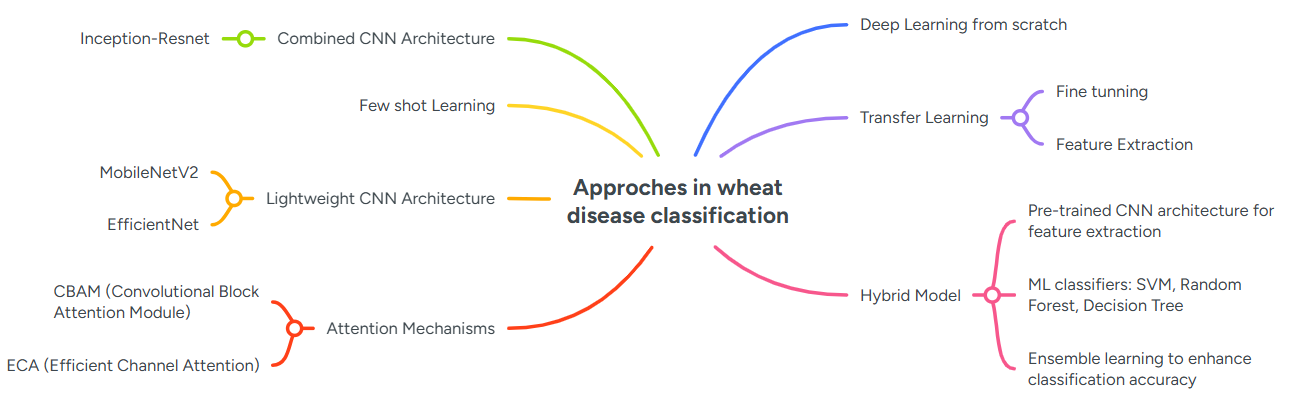
\includegraphics[width=1.0\textwidth]{chapters/chapter3/images/Figure09.png}
    \caption{Taxonomy of Approaches for Classifying Wheat Diseases. \protect\parencite{haider2021wheat}}
    \label{fig:Figure01}
\end{figure}


\section{Core Limitations and Research Gaps in Wheat Disease and Pest Detection}
Deep learning has shown great promise in automating wheat disease detection, offering timely and precise solutions for sustainable agriculture. However, key challenges still limit its widespread adoption.

Based on the previously discussed studies, various approaches have been explored for wheat disease classification, ranging from transfer learning using pre-trained convolutional neural networks (CNNs) to the development of custom architectures tailored specifically for disease classification tasks. The proposed models for wheat disease classification that detect five or fewer disease classes generally achieve accuracies of 99% or higher. However, models aiming to detect more than five classes tend to achieve lower accuracies, typically below 98%, highlighting the challenge of achieving high accuracy when dealing with more complex classification tasks.

Additionally, the number of disease classes addressed in most proposed models for wheat detection remains limited compared to the actual variety of diseases observed in the field, with a maximum of five classes, primarily due to the difficulty of manual annotation and the high computational resources required to train models on larger, more diverse datasets. Although several public datasets for wheat disease classification are available, such as those on Kaggle, these sources often contain low-quality images, inconsistent labeling, or irrelevant data, which can hinder model training and performance. This necessitates manual cleaning and preprocessing of the datasets before they can be effectively utilized, increasing the time and effort needed for research.

Moreover, the performance of these models is often affected by inconsistencies in image data. Therefore, diversifying image data is crucial; photos should be taken under varying lighting conditions, such as on sunny and cloudy days, and from different distances, including both close-up and wider shots. Creating a custom dataset by selecting diverse images from different public datasets is important to ensure this variability and improve model robustness.

Beyond dataset issues, several structural and architectural limitations remain. Most current models use a single-stage classification pipeline that attempts to identify all classes in one pass. This approach can be inefficient, especially when simple distinctions (e.g., healthy vs. diseased) could be resolved earlier using lightweight inference mechanisms. The lack of hierarchical or multi-stage classification pipelines presents an opportunity for improvement in computational efficiency and deployment readiness.

Furthermore, few models explicitly address deployment constraints such as low computational power, memory limitations, or real-time processing requirements, which are crucial for applications in edge computing or mobile agricultural tools used directly in the field. The absence of design considerations for lightweight architectures and early-exit strategies limits the practical applicability of many existing solutions.

Another significant limitation is the lack of evaluation on real-world field images that exhibit high variability in terms of background, illumination, occlusion, and resolution. While many models achieve excellent performance on curated datasets, their generalization to uncontrolled field conditions remains underexplored. Robustness under such conditions is essential for real-life adoption by farmers and agronomists.

Finally, although attention mechanisms and hybrid models have been proposed in recent literature, few studies explicitly quantify the trade-offs between accuracy and computational cost in multi-class settings, especially when scaling up to cover a wider range of diseases.

\section{Conclusion}
While deep learning has shown strong potential in wheat disease detection, a major limitation across current studies is the restricted number of disease classes addressed—often no more than five. This narrow scope limits the practical applicability of these models in real agricultural environments, where a wider range of diseases must be identified accurately. The difficulty of collecting and annotating diverse, high-quality images, along with the computational cost of training on large-scale multi-class datasets, remains a significant barrier. Additionally, many existing models struggle to maintain high accuracy when scaled to include more disease categories.

These challenges highlight the need for systems capable of handling a greater number of classes without compromising accuracy. In the next chapter, we present the design and implementation of our proposed solution, which is specifically developed to support accurate multi-class classification and improved generalization to real-world conditions.